\documentclass[parskip=half]{scrartcl}

\usepackage{amsmath}
\usepackage{mathtools}
\usepackage{graphicx}
\usepackage{hyperref}
\usepackage[textsize=tiny]{todonotes}
\graphicspath {{images/}}
\hypersetup{
    colorlinks=true,
    citecolor=blue
}

\begin{document}

\title{CS698 (Winter 2017) Notes}
\author{Vineet John (v2john@uwaterloo.ca)}
\date{\today}
\maketitle

\section{Supervised Learning}\label{supervised-learning}

    Classification: domain of output is categorical (discrete)\\
    Regression: domain of output is numerical (continuous)

    Input domain can be either discrete or continuous for both.

    Examples:\\
    Appln - Domain - Range - Type of Problem\\
    Spam Identification - Words/Characters - spam/ham - classification\\
    Stock Prices - Prev price/news - predicted value - regression\\
    Speech recognition - Audio signal - words - classification\\
    Digit recognition - Image - Digits - classification\\
    Housing value - Area/bedrooms/baths - market value - regression\\
    Weather prediction - Local weather/Prev weather - Temp/Rain - Regression/Classificn

    Consider space of probably hypotheses\\
    Approximation of a best solution is done within this space\\
    A good hypothesis generalizes well

    When is it not possible to find a consistent hypothesis

    \begin{itemize}
        \item
        Insufficient Hypothesis space
        \item
        Noise in the training data
    \end{itemize}

    Tradeoff: Expressiveness vs complexity in finding a hypothesis - in the
    hypothesis space

\section{Statistical Learning}\label{statistical-learning}

    \begin{itemize}
        \item
        Joint probabilities
        \item
        Marginalization - sum up a join probability over a variable to express
        it in terms of another variable
        \item
        Conditional probabilities i.e A, given B
        \item
        Conditional probabilies need not sum up to 1, since the idea of a
        context is introduced.
    \end{itemize}

    \subsection{Bayes Rule}\label{bayes-rule}

    \begin{itemize}
        \item
        Posterior probabiliy = prediction, Prior = hypothesis, evidence =
        input variables, likelihood = probability of evidence given the prior
        hypothesis
        \item
        Weigh each hypothesis and use all hypothesis to get an avg prediction
        \item
        No overfitting, all hypotheses considered and weighed according to
        their probabilities
    \end{itemize}


\section{Logistic Regression}
\label{logistic-regression}

    \subsection{Overview - Logistic Regression} % (fold)
    \label{sub:overview_logistic_regression}
    \begin{itemize}
        \item 
        In Mixture of Gaussians, we learn the prior and the likelihood and used Bayesian learning to compute the posterior.
        \item 
        Unlike Mixture of Gaussians, we learn the posterior directly by maximum likelihood
    \end{itemize}

    % subsection overview_logistic_regression (end)

    \subsection{Problem - Singular Hessian}\label{problem---singular-hessian}

    \begin{itemize}
        \item
        Attempt is to make the ridge of the sigmoid function as shape as
        possible
        \item
        When weights tend to negative infinity, the sigmoid function tends to
        zero
        \item
        As the sigmoid is a component of the hessian, the hessian diagonal
        then is comprised of zeoes.
        \item
        This could result in the Hessian becoming a singular matrix
    \end{itemize}

    \subsection{Solutions}\label{solutions}

    \begin{itemize}
        \item
        Adding a penalty term to the loss function
        \item
        Boils down to adding a magnified identity matrix to the Hessian
    \end{itemize}

\section{Generalized Linear models}\label{generalized-linear-models}

    \begin{itemize}
        \item
        Mapping the input space into a lower dimensional space
        \item
        Perform linear regression of the dataset
        \item
        Polynomial class of functions used as basis functions.
        \item
        Basis functions are used for the mapping
        \item
        The input space x is mapped as $\Phi(x)$
    \end{itemize}


\newpage


\section{Perceptron \& Neural Nets}\label{perceptron-neural-nets}

    \begin{itemize}
        \item
        Output in the form of a non-linear function
        \item
        A neuron produces a single output, which may, in turn, be fed to
        multiple other neurons.
        \item
        Types of activation function:

        \begin{itemize}
            \item
            Threshold: Step function, non-linear
            \item
            Sigmoid: Smoother version of the step function
        \end{itemize}
        \item
        Nets can be trained by tuning the weights.
    \end{itemize}

    \section{Threshold Perceptron Learning}\label{threshold-perceptron-learning}

    \begin{itemize}
        \item
        Add/subtract the input vector to/from the weights if the predicted
        value doesn't match the target.
        \item
        Eta determines the magnitude of the step-size
        \item
        Gradient descent: Assuming threshold perceptron, will converge if data
        is linearly separable.
        \item
        If the data isn't linearly separable

        \begin{itemize}
            \item
            The algorithm will never converge
            \item
            The step vector keeps being reset back \& forth
        \end{itemize}
    \end{itemize}

    \section{Sigmoid Perceptron}\label{sigmoid-perceptron}

    \begin{itemize}
        \item
        Similar to logistic regression in that it computes a sigmoid
        separator.
        \item
        Multiple sigmoid hyperplanes could be used to simulate a ridge-like
        hyperplane. Further compounding can lead to simulating a bump-like
        hyperplane.
    \end{itemize}

    \section{Multi-layer neural networks}\label{multi-layer-neural-networks}

    \begin{itemize}
        \item
        Mapping inputs into a linear feature space, and then applying linear
        learning algorithms like linear regression, threshold functions,
        mixtures of gaussians and logistic regression.
        \item
        A neural net could be used to approximately just about any function
        using a combination of neurons.
    \end{itemize}

    \subsection{Feedforward neural
    network}\label{feedforward-neural-network}

    \begin{itemize}
        \item
        Adaptive non-linear basis function = function chaining
    \end{itemize}

    \section{Multi-Layer Neural Nets}\label{multi-layer-neural-nets}

    \begin{itemize}
        \item
        Sequential gradient descent used, similar to a gradient descent
        approach for linear regression.
        \item
        Backpropagation permits simultaneous calculation of weights for the
        perceptrons in a multi-layered neural network.
        \item
        Involves a forward and a backward phase.
        \item 
        The forward phase calculates the output $z_j$ for each unit $j$
        \item
        The backward phase propagates errors to the input units, error denoted
        by $\delta_j$ at each unit $j$
    \end{itemize}

    Neural net = composition of functions
    \begin{itemize}
        \item
        Decompose the derivative of the error function, using the chain rule
        \item
        $w_{ij}$ is the weight metric from unit i to unit j
        \item
        $\delta_{ij}$ is the error metric from unit j to unit i
        \item
        Example using tanh as a hypothesis function to calculate the
        activation weights
    \end{itemize}


\newpage


\section{Kernel methods}\label{kernel-methods}

    \begin{itemize}
        \item
        Avoids the complexity of convex optimization
        \item
        Kernel Trick - Related to duality
        \item
        Derived from the dot product of the input and it's embedding into a
        new feature space.
    \end{itemize}

    \subsection{Generalized linear
    functions}\label{generalized-linear-functions}

    \begin{itemize}
        \item
        Fixed non-linear basis functions
        \item
        Limited hypothesis space
        \item
        Easier to optimize
    \end{itemize}

    \subsection{Neural networks}\label{neural-networks}

    \begin{itemize}
        \item
        Adaptive non-linear basis functions
        \item
        Rich hypothesis space
        \item
        Difficult to opitimize (by virtue of being non-convex)
    \end{itemize}

    \section{Kernel methods (contd.)}\label{kernel-methods-contd.}

    \begin{itemize}
        \item
        Rather than trying to compute the function $\Phi$, the
        objective is to be able to start with an arbitrary Gram matrix.
        \item
        Slide 10 - dimensionality of each vector is 2. The square function is
        the new space than the gram matrix can emulate by computing the dot
        product of the x vector and the z vector.
        \item
        Gaussian kernel is unrelated to the PDF of a gaussian distribution.
        \item
        Primal solution - scales with the number of basis functions
        \item 
        Dual solution - scales with data
        \item 
        A valid kernel must has non-zero eigenvalues, if it's being guessed rather than computed
    \end{itemize}


\newpage


\section{Gaussian Processes} % (fold)
\label{sec:gaussian_processes}
\begin{itemize}
    \item
    Uncertainty in the weights for a linear regressor can be translated into a corresponding uncertainty for the output space. Both are modeled as Gaussian distributions.
    \item
    Continuous functions implies that there are infinite Gaussian distributions that describe the output space.
    \item
    Kernel function is used as a covariance matrix to indicate that the Gaussian distribution of the output space is very similar for points that are closely-correlated.
    \item 
    Describes a distribution over each point in the target function. 
    \item 
    Bayesian Learning used to learn a posterior distribution of what the Gausian processes look like.
    \item 
    Function space view: Scales with the amount of data rather than the number of dimensions. Useful for problems where the dimensions might be infinitely many. The weight space view applies to the opposite scenario.
    \item 
    Example of Gait Optimization shown in Figure \ref{fig:gait_optimization}.
    \begin{itemize}
        \item 
        Experimentation done using new feature vectors (denoted by $X_{new}$).
        \item 
        Minimizes the magnitude of the Gaussian deviation.
        \item 
        Iteratively run new experiments with different values of $X_{new}$ to converge to a result.
    \end{itemize}
    \begin{figure}[th]
    \centering
    \includegraphics[width=0.6\textwidth]{gait_optimization}
    \caption{Gait Optimization}
    \label{fig:gait_optimization}
    \end{figure}
\end{itemize}

% section gaussian_processes (end)


\newpage


\section{Support Vector Machines} % (fold)
\label{sec:support_vector_machines}

    \subsection{Overview - SVM} % (fold)
    \label{sub:overview_svm}

    \begin{itemize}
        \item 
        Also uses kernel trick, but the kernel uses a subset of the data.
        \item 
        SVM attempt to maximize the margin between the support vectors and the hyperplane. Ref Figure \ref{fig:svm_general}
        \begin{figure}[th]
        \centering
        \includegraphics[width=0.4\textwidth]{svm_general}
        \caption{SVM Diagram}
        \label{fig:svm_general}
        \end{figure}
        \item 
        SVMs are also called max-margin classifiers. $a > b$ in Figure \ref{fig:max_margin}
        \begin{figure}[th]
        \centering
        \includegraphics[width=0.4\textwidth]{max_margin}
        \caption{Max margin}
        \label{fig:max_margin}
        \end{figure}
        \item 
        $w^T \Phi(x) = 0$ represents the linear separator
        \item 
        Dividing by $\Vert w\Vert$ ensures that the distance to the linear separator is normalized in terms of unit length.
        \item 
        The problem is made tractable in terms of the data by relying only on the support vectors while performing the quadratic optimization.
        \item 
        The quadrative objective is reformulated as a dual representation in $\Phi(x)$
        \item 
        The result is an optimization objective in the auxilliary variable $a$, which is the weight for the penalty term. $a_n = 0$ for any data-points apart from the support vectors.
    \end{itemize}    
    % subsection overview_svm (end)

    \subsection{Overlapping classes and slack variables} % (fold)
    \label{sub:overlapping_classes_and_slack_variables}

    \begin{itemize}
        \item $\epsilon$ parameterized the soft-margin which is an allowance for some data point to lie beyond the margin.
        \item If misclassfied, $\epsilon > 1$.\\ If within the soft margin, $1 > \epsilon > 0$.\\ If on the margin, $\epsilon = 0$\\
        Refer to figure \ref{fig:soft_margins}
        \begin{figure}[ht]
            \centering
            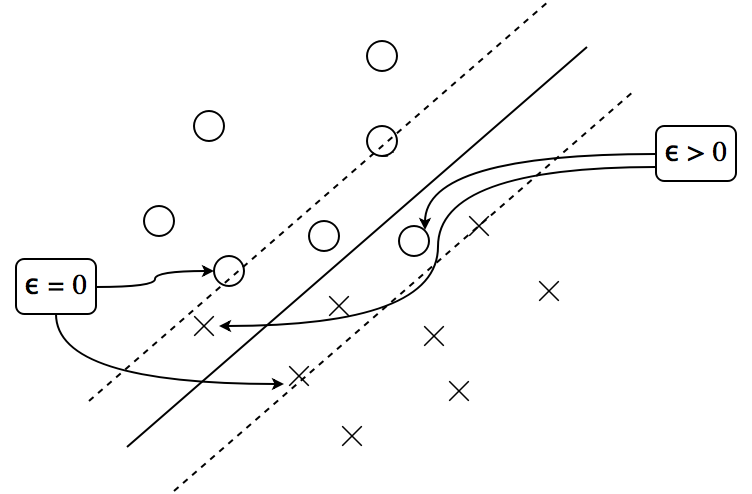
\includegraphics[width=0.4\textwidth]{soft_margins.png}
            \caption{Soft Margins - SVM}
            \label{fig:soft_margins}
        \end{figure}
        \item $C$ controls how much to weigh vanilla SVMs over the new optimization problem for soft margins. Hard margin classifier implies that we're assuming the data is linearly separable.
        \item For the new optimization problem, earlier only support vectors were considered, but now, we consider points on the margin, points within the margin as well as misclassified points.
        \item Computation complexity increases as the number of vectors increase.
    \end{itemize}
    
    % subsection overlapping_classes_and_slack_variables (end)

    \subsection{Muticlass SVMs} % (fold)
    \label{sub:muticlass_svms}
    \begin{itemize}
        \item One vs Rest, for all classes, then combine. 
            \begin{figure}[ht]
                \centering
                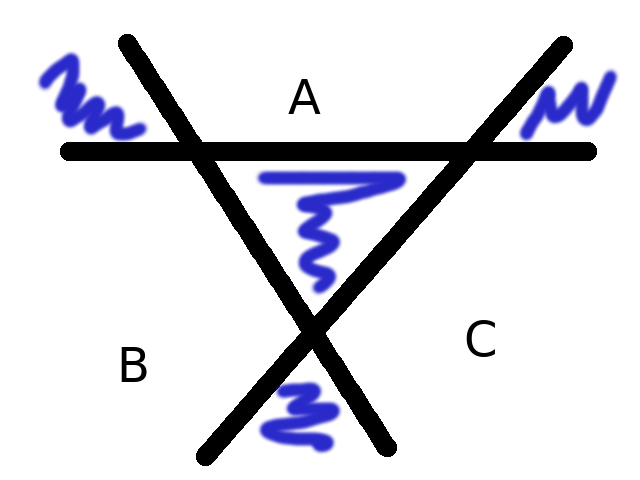
\includegraphics[width=0.4\textwidth]{one_vs_all_and_pairwise.png}
                \caption{One vs. All / Pairwise}
                \label{fig:one_vs_all_and_pairwise}
            \end{figure}
            Shaded regions are uncertain
        \item Pairwise comparison - exhaustive
            Similar to the prev. SVM, there are areas of uncertainty between classes.
        \item Continuous ranking - Best ranked
            \begin{figure}[ht]
                \centering
                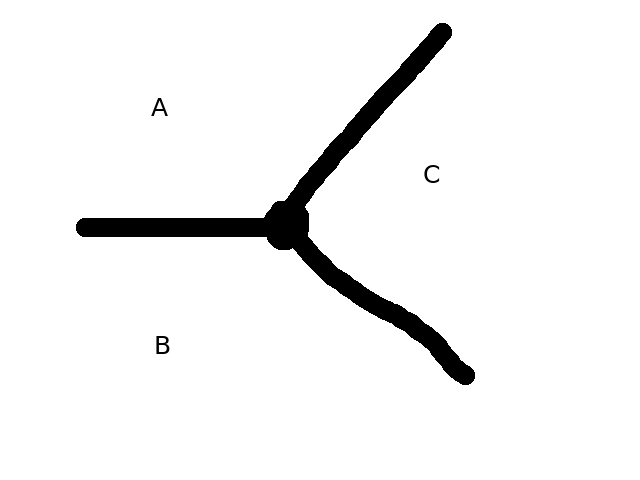
\includegraphics[width=0.4\textwidth]{continuous_rank_svm.png}
                \caption{Continuous Ranking}
                \label{fig:continuous_rank_svm}
            \end{figure}
            No uncertainty as we pick the highest ranked class.
            This needs a vector $w$ to define the hyperplane for each class. where $w$ represents the distance of a point to the separating hyperplane.
    \end{itemize}
    % subsection muticlass_svms (end)

    \subsection{Multi-class Classification} % (fold)
    \label{sub:multi_class_classification}
    \begin{itemize}
        \item Multi-class expression is a generalization of the binary SVM expression.
        \item The concept of soft-margins can also be applied here.
    \end{itemize}
    % subsection multi_class_classification (end)

    \subsection{Comparison to Perceptrons} % (fold)
    \label{sub:comparison_to_perceptrons}

    Perceptrons:
    \begin{itemize}
        \item 
        Linear separator - depends on starting values
        \item 
        Simple update rule
        \item 
        Prone to over-fitting
    \end{itemize}

    Support vector machines
    \begin{itemize}
        \item 
        Unique max-margin linear separator
        \item 
        Quadratic optimization
        \item 
        Robust to over-fitting
    \end{itemize}
    
    % subsection comparison_to_perceptrons (end)

% section support_vector_machines (end)


\newpage


\section{Hidden Markov Models} % (fold)
\label{sec:hidden_markov_models}

    \subsection{Overview - Hidden Markov Models} % (fold)
    \label{sub:overview_hidden_markov_models}
        
        \begin{itemize}
            \item Data-points are not always IID. Context taken into account while predicting current value.
            \item Correlation with the prior data-points are leveraged.
            \item Stationary assumption: Assumes that the correlation between 2 output variables remains constant over the output space.
            \item Emission - $P(x|y)$, Transition - $P(y_t, y_{t-1})$
            \item Both the emission and transition are defined in terms of multinomial (discrete) distributions. e.g. values of a dice
            \item Joint Distribution - $P(y_{1..t}, x_{1..t}) = P(y_i) \prod_i P(x_i|y_i) \prod_i P(y_i|y_{i-1}) $
            \item Example - cascading uncertainty for a robot's movements over time.
            \item HMM Problem: $P(y_t|x_t .. x_1) $
        \end{itemize}

    % subsection overview_hidden_markov_models (end)

    \subsection{Applications of HMMs} % (fold)
    \label{sub:applications_of_hmms}

        \textbf{Monitoring}
        \begin{itemize}
            \item Predicting the current output state given a historical set of inputs.
            \item Can be expressed in terms of a recursive algorithm, that will required the output classes of the previous epochs.
            \item Forward algorithm - computes from the 0th epoch. Linear complexity in the number of epochs.
        \end{itemize}

        \textbf{Prediction/Forecasting}
        \begin{itemize}
            \item Similar approach to monitoring. Can be expressed recursively.
        \end{itemize}

        \textbf{Hindsight}
        \begin{itemize}
            \item Computing the output class at a given epoch, given input observations in the past and future. $1 < k < t$
            \item Forward-backward algorithm - uses epochs $1..k$ in the forward phase and $k..t$ in the backward phase.
        \end{itemize}

        \textbf{Most likely explanation}
        \begin{itemize}
            \item Predict entire sequence of output class $y_1..y_t$. Can be used in the context of speech recognition.
        \end{itemize}

        Viterbi algorithm - dynamic programming formulation. Discrete distribution of the output class y depends on the Initial State ($\pi$), Transition ($\theta$) and Emission ($\phi$)

        \textbf{Example}
        \begin{itemize}
            \item 2 classes - walking($c_1$) and sitting ($c_2$)
            \item input measurements (accelerometer) - high ($v_1$) and low ($v_2$)
            \item 100 training experiments
            \item 
                Statistics
                \begin{itemize}
                    \item $\#c_1^{start} = 90$, $\#c_2^{start} = 10$
                    \item $\#(c_1, c_1) = 80000$, $\#(c_2, c_1) = 20000$
                    \item $\#(c_1, c_2) = 10000$, $\#(c_2, c_2) = 90000$
                    \item $\#(v_1, c_1) = 75000$, $\#(v_2, c_1) = 25000$
                    \item $\#(v_1, c_2) = 30000$, $\#(v_2, c_2) = 70000$
                    \item $P(y_{start} = c_1) = 0.9$, $P(y_{start} = c_2) = 0.1$
                    \item Frequency of starting with a particular class
                        \begin{itemize}
                            \item Transition
                            \begin{table}[ht]
                                \centering
                                \begin{tabular}{| l | c c |}
                                    \hline
                                    \textbf{} & \textbf{$c_1$} & \textbf{$c_2$} \\
                                    \hline\hline
                                        $c_1$ & 0.8 & 0.2 \\
                                    \hline
                                        $c_2$ & 0.1 & 0.9 \\
                                    \hline
                                \end{tabular}
                                \caption{Transition Probabilities}
                                \label{tab:transition_probabilities}
                            \end{table}
                            \item Emission
                            \begin{table}[ht]
                                \centering
                                \begin{tabular}{| l | c c |}
                                    \hline
                                    \textbf{} & \textbf{$v_1$} & \textbf{$v_2$} \\
                                    \hline\hline
                                        $c_1$ & 0.75 & 0.25 \\
                                    \hline
                                        $c_2$ & 0.3 & 0.7 \\
                                    \hline
                                \end{tabular}
                                \caption{Emission Probabilities}
                                \label{tab:emission_probabilities}
                            \end{table}
                        \end{itemize}
                \end{itemize}
        \end{itemize}

        \textbf{Forward algorithm - Example of Monitoring}
        \begin{itemize}
            \item Input set is $[v_1, v_1, v_2, v_2]$. Could be accelometer readings.
            \item $P(y_1|v_1) \propto P(v_1|y_1)P(y_1) = [0.675, 0.03] \propto [0.9574,  0.0426] (normalized) $
            \item $P(y_2|v_1, v_1) \propto P(v_1|y_2) \sum_{y_1} P(y_2|y_1) P(y_1|v_1) = [0.5809, 0.0402] \propto [0.9553, 0.0647] (c_1, c_2) $
            \item $P(y_3|v_1, v_1, v_2) \propto P(v_3|y_3) \sum_{y_2} P(y_3|y_2) P(y_2|v_1, v_1) = [0.1903, 0.1063] \propto [0.6417, 0.3583] $
            \item $P(y_4|v_1, v_1, v_2, v_2) \propto P(v_4|y_4) \sum_{y_3} P(y_4|y_3) P(y_3|v_1, v_1, v_2) = [0.1463, 0.2707] \propto [0.3308, 0.6492] $
        \end{itemize}
        
        \textbf{Most likely explanation - Example}
        \begin{itemize}
            \item 
            $$f(y_1, y_2) = P(y_2|y_1) P(v_1|y_1) P(y_1)$$
            $$[y_1 = c_1, y_1 = c_2] [y_2 = c_1, y_2 = c_2] = [[0.54, 0.135], [0.003, 0.027]] $$
            $$\max_{y_1} P(y_1y_2|v_1) = \max_{y_1} f(y_1, y_2) = [0.54, 0.135] $$
            \item 
            $$f(y_2, y_3) = P(y_3|y_2) P(v_1|y_2) \max_{y_1} P(y_1y_2|v_1)$$
            $$[y_2 = c_1, y_1 = c_2] [y_3 = c_1, y_2 = c_2] = [[0.324, 0.081], [0.0041, 0.0345]] $$
            $$\max_{y_1y_2} P(y_1y_2y_3|v_1v_1) = \max_{y_2} f(y_2, y_3) = [0.324, 0.081] $$
            \item 
            $$f(y_3, y_4) = P(y_4|y_3) P(v_2|y_3) \max_{y_1y_2} P(y_1y_2y_3|v_1v_1)$$
            $$[y_3 = c_1, y_1 = c_2] [y_4 = c_1, y_2 = c_2] = [[0.0648, 0.0162], [0.0057, 0.0310]] $$
            $$\max_{y_1y_2y_3} P(y_1y_2y_3y_4|v_1v_1v_2) = \max_{y_3} f(y_3, y_4) = [0.0648, 0.051] $$
            \item 
            $$f(y_4) = P(v_2|y_4) \max_{y_1y_2y_3} P(y_1y_2y_3y_4|v_1v_1v_2)$$
            $$[y_4 = c_1, y_4 = c_2] = [0.0162, 0.357] $$
            $$\max_{y_1y_2y_3y_4} P(y_1y_2y_3y_4|v_1v_1v_2v_2) \propto \max_{y_4} f(y_4) = 0.0357 $$
        \end{itemize}

    
    % subsection applications_of_hmms (end)

% section hidden_markov_models (end)

\newpage


\section{Deep Neural Networks} % (fold)
\label{sec:deep_neural_networks}

    \begin{itemize}
        \item 
        Example of scaling w.r.t. depth of the network as opposed to a single hidden layer (Parity function.)
        \item 
        Most popular activation functions for units - sigmoid (0 to 1) and tanh (-1 to 1)
        \item 
        \textbf{Vanishing gradient}
        \begin{itemize}
            \item 
            Vanishing gradient problem: Appearing to converge too soon. Gradient might not result in any change in the initial layers after backpropagation.
            \item 
            Sequential squashing of the gradient results in gradually vanishing over time. Chain rule results in multiplying multiple numbers between 0 and 1, which could lead to computing a gradient below the required threshold to take a step in the direction of the minima of the convex function.
            \item 
            Compounded product of the output value ranges over multiple layers resultings in the gradient converging to 0. This is because both the output and the gradient for both logistic sigmoid units and hyperbolic tan units are always between 0 and 1 in terms of magnitude.
            \item 
            Possible solutions include 
            \begin{itemize}
                \item 
                Using a larger gradient for the layers close to the output layer.
                \item 
                Using pre-trained units.
                \item 
                Using recitified linear units.
            \end{itemize}
        \end{itemize}
    \end{itemize}

    \subsection{Rectified Linear Units} % (fold)
    \label{sub:rectified_linear_units}
    
    \begin{itemize}
        \item 
        $h(a) = max(0, a) $
        \item 
        Softplus: $h(a) = log(1 + e^a) $, where $a = \sum_i w_i x_i $
        \item 
        If gradient is negative, don't back-propagate, if not, then set gradient to 1. This ensures that the gradient doesn't vanish for pathways in the network with $a > 0$.
        \item 
        Softplus might also result in a vanishing gradient if the network has several layers.
        \item 
        The disadvantage of using the rectified linear function is that it only approximately a linear function at most. Piecewise linear function (Figure \ref{fig:piecewise-linear-function}). 
        \begin{figure}[ht]
            \centering
            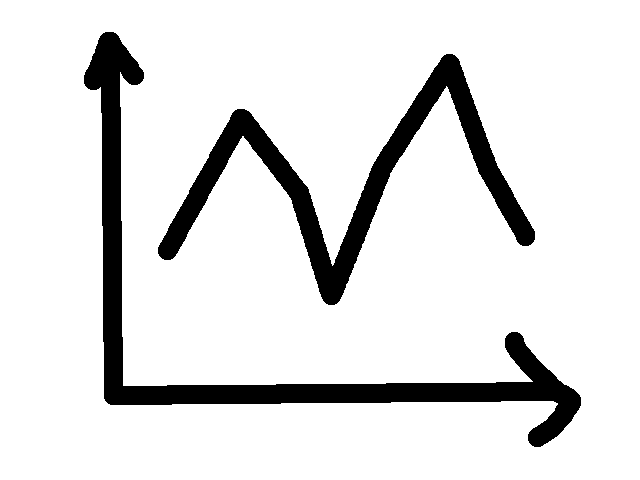
\includegraphics[width=0.4\textwidth]{piecewise-linear-function}
            \caption{Piecewise Linear Function}
            \label{fig:piecewise-linear-function}
        \end{figure}
    \end{itemize}

    % subsection rectified_linear_units (end)

    \subsection{Maxout Units} % (fold)
    \label{sub:maxout_units}

        \begin{itemize}
            \item Maxout Unit (Figure \ref{fig:maxout-unit})
            \begin{figure}[ht]
                \centering
                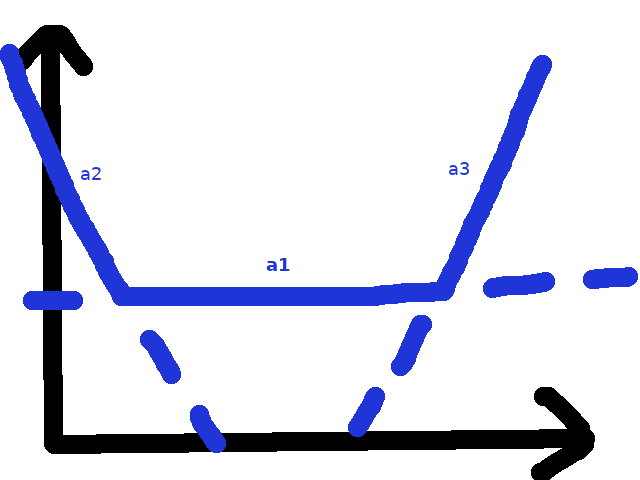
\includegraphics[width=0.4\textwidth]{maxout-unit}
                \caption{Maxout Unit}
                \label{fig:maxout-unit}
            \end{figure}
            \item 
            Choose $a$ such that $a = max(a_1, a_2, a_3)$, where $a_{ij} = \sum_j w_{ij} z_j $
            \item 
            Produces a piecewise linear function, which is also convex.
        \end{itemize}
    
    % subsection maxout_units (end)

    \subsection{Overfitting} % (fold)
    \label{sub:overfitting}

    \begin{itemize}
        \item 
        Due to high expressivity, the data could be very easily overfit.
        \item 
        Solutions:
        \begin{itemize}
            \item 
            Regularization: Penalizing large weights
            \item 
            Data augmentation: Minor variations in the input data to allow the network to train a model that is invariant to small changes in the input data.
            \item 
            Dropout: Randomly drop some units from the network during the training phase. Intended to increase network robustness against overfitting to specific datapoints.\\
            Dropout can be viewed as an approximation ensemble learning. Units need to stay in memory for this to work.
        \end{itemize}
    \end{itemize}
    
    % subsection overfitting (end)
    
% section deep_neural_networks (end)



\section{Convolutional Neural Networks} % (fold)
\label{sec:convolutional_neural_networks}

    \begin{itemize}
        \item 
        Convolution: A mathematical operation on two function that produced a third, which can be viewed as a modified version of one of the initial two functions.
        \item 
        Example of convolution: smoothing a function. (Figure \ref{fig:cnn-smoothing})
        \begin{figure}[ht]
            \centering
            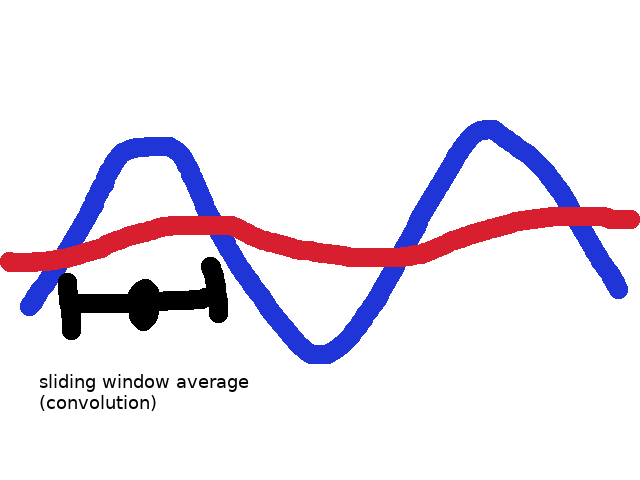
\includegraphics[width=0.4\textwidth]{cnn-smoothing}
            \caption{Smoothing function - convolution}
            \label{fig:cnn-smoothing}
        \end{figure}
        \item 
        $x$, the original input, is multiplied by a weight factor $w$ to obtain an output (either discrete or continous)
        \item 
        Image example: white-to-black produces a black edge and vice-versa. Simple convolution.
        \item 
        Could also be used for feature extraction when combined with an activation function.
        \item 
        A convolution is a linear subset of units based on a specific weight vector.
        \item 
        Activation functions confirm the existence of a patter.
        \item 
        Gabor filters: Base weights used for image recognition. Comparisons against them could be use to detect patterns via convolutions.
        \item 
        Architecture: Comprised of alternating convolutional and pooling layers. (Figure \ref{fig:cnn-arch})
        \begin{figure}[ht]
            \centering
            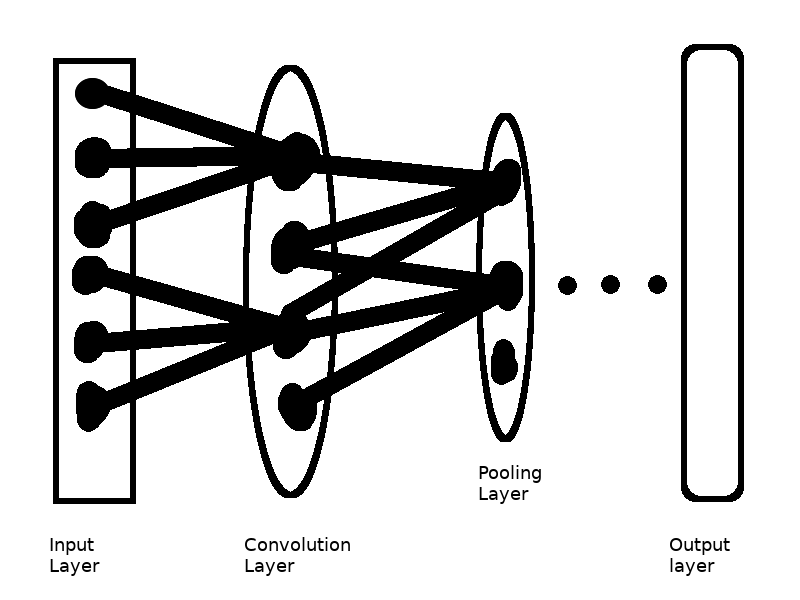
\includegraphics[width=0.4\textwidth]{cnn-arch}
            \caption{CNN Architecture}
            \label{fig:cnn-arch}
        \end{figure}
        \item 
        Pooling: Aggregating the output of the result of the convolutional layer. It could be using a max/sum/avg function.
        \item 
        A max pooling function could simulate an invariant i.e. doesn't matter which section of a given patch a pattern is found in.
        \item 
        Pooling function is typically a commutative math operator.
    \end{itemize}


    \subsection{CNN Properties} % (fold)
    \label{sub:cnn_properties}
    
        \begin{itemize}
            \item 
            CNNs won't usea fully connected network. Connections are sparse because only contiguous patches of the image are considered as input features to the convolutional layers.
            \item 
            Weights are the same across a single layer, so the fact that they are shared simplifies the network.
        \end{itemize}

    % subsection cnn_properties (end)

    \subsection{MNIST CNN Example} % (fold)
    \label{sub:mnist_cnn_example}

        \begin{itemize}
            \item 
            32x32 images, 5x5 patches as features for the convolutional layer, resulting in an abstracted 28x28 input space. Pooling layer of 2x2 dimensions, which means that every 4 units is pooled, reducing the feature space to a 14x14 space.
            \item 
            This 14x14 is now treated as the original 32x32 image, and recursively worked on by alternating convolutional and pooling layers.
        \end{itemize}
    
    % subsection mnist_cnn_example (end)

% section convolutional_neural_networks (end)


\newpage


\section{Recurrent/Recursive Neural Networks} % (fold)
\label{sec:recurrent_recursive_neural_networks}

    \begin{itemize}
        \item 
        Typically used when the input data is comprised of sequences, time series, textual data.
        \item 
        Weights are shared across time steps.
        \item 
        Unit representation: (Figure \ref{fig:rnn-units})
        \begin{figure}[ht]
            \centering
            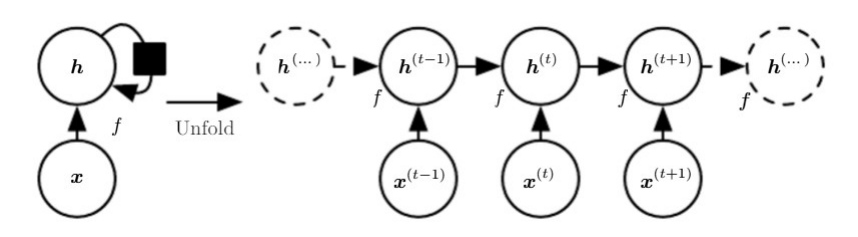
\includegraphics[width=0.4\textwidth]{rnn-units}
            \caption{RNN Units}
            \label{fig:rnn-units}
        \end{figure}
        \item 
        Errors tend to cascade in RNNs, as they are based on sequential data. The errors might also be compounded.
        \item 
        HMMs can be a specific implementation of an RNN. 
        Belief monitoring can be done as shown below. Figure \ref{fig:rnn}
        $P(Y_1|X_1)$ could be computed as either the sigmoid or softmax (binary/categorical outputs), or a Gaussian distribution (continuous outputs)
        \begin{figure}[ht]
            \centering
            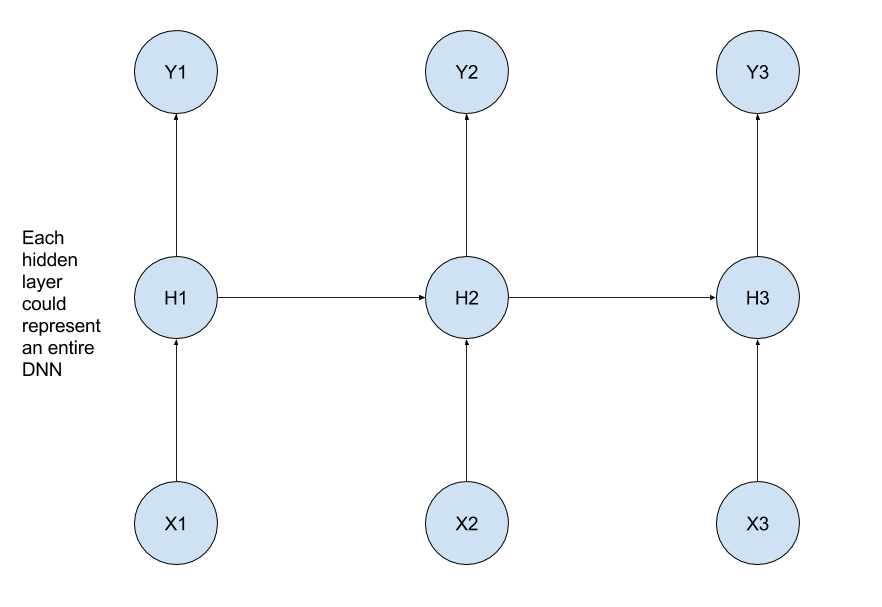
\includegraphics[width=0.7\textwidth]{rnn}
            \caption{RNN - Belief Monitoring}
            \label{fig:rnn}
        \end{figure}
        \item 
        Prediction cannot be done since the output $y$ at a given time-step depends on it's input at the same step.
        \item 
        HMM: more flexible queries\\
        RNN: more expressive distributions
    \end{itemize}


    \subsection{Bi-directional RNN} % (fold)
    \label{sub:bi_directional_rnn}
        \begin{itemize}
            \item Hindsight queries : Figure \ref{fig:bi-directional_rnn}
            \begin{figure}[ht]
            \centering
            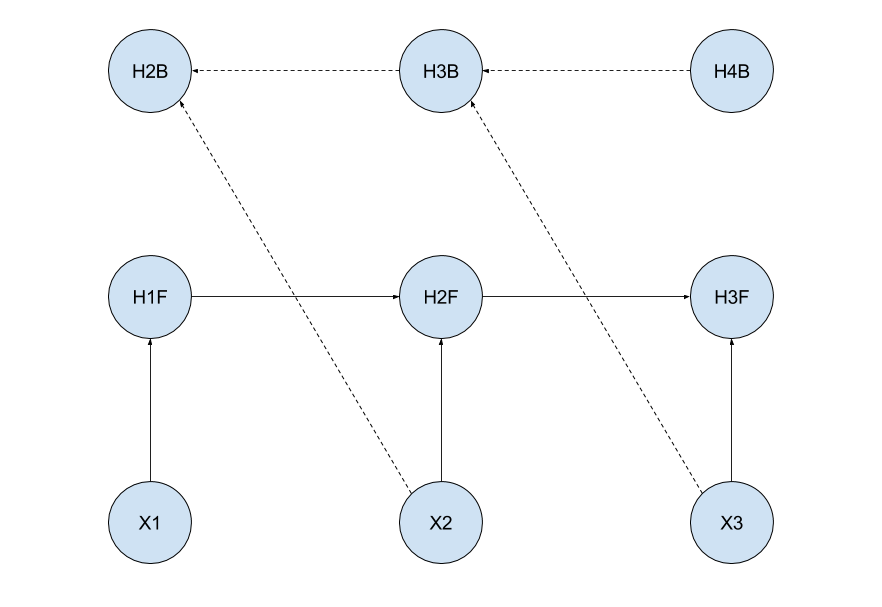
\includegraphics[width=0.7\textwidth]{bi-directional_rnn}
            \caption{Bi-directional RNN - Hindsight queries}
            \label{fig:bi-directional_rnn}
        \end{figure}
            \item 
            $P(y_2| x_1, x_2, x_3, x_4)$ is an example of a hindsight prediction that can be made using bi-directional RNNs.
        \end{itemize}
    % subsection bi_directional_rnn (end)

    \subsection{Encoder - Decoder Model} % (fold)
    \label{sub:encoder_decoder_model}

        \begin{itemize}
            \item 
            \textbf{Usage in Machine translation:}
            \begin{itemize}
                \item 
                Encoding sentences into a vector representation.
                \item 
                The encoded segment is the context.
                \item 
                While decoding, each step in the model stores what the network has translated thus far, the output for this is the word in the new language.
            \end{itemize}
        \end{itemize}
    
    % subsection encoder_decoder_model (end)

    \subsection{Recursive Neural Networks} % (fold)
    \label{sub:recursive_neural_networks}

        \begin{itemize}
            \item 
            Generalize recurrent neural networks from chains to trees.
            \item 
            Useful to identify vector representation of variable length data.
            \item 
            Applications for Semantic Parsing. Figure \ref{fig:dependency-parser}
            \begin{figure}[ht]
                \centering
                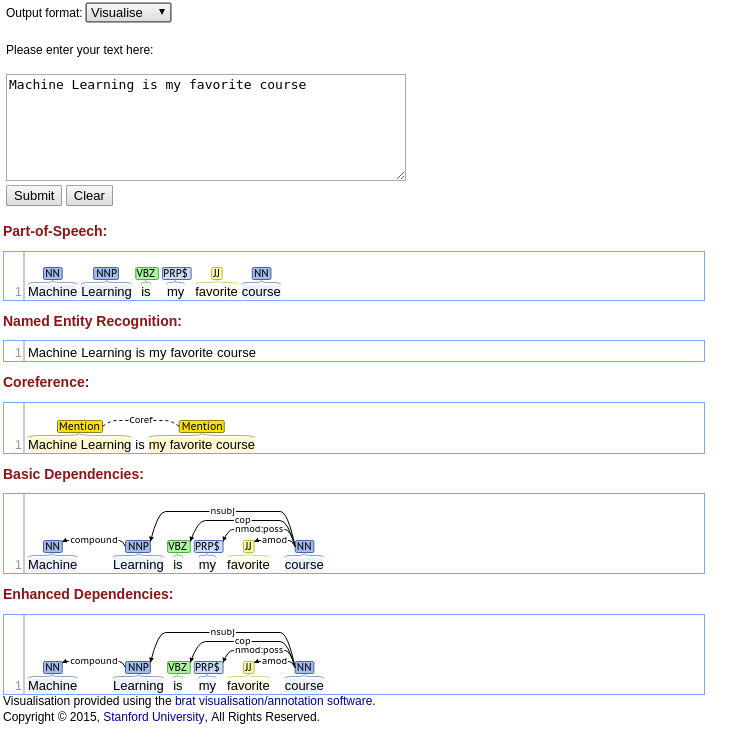
\includegraphics[width=0.7\textwidth]{dependency-parser}
                \caption{Dependency Parsing}
                \label{fig:dependency-parser}
            \end{figure}
        \end{itemize}
    
    % subsection recursive_neural_networks (end)

    \subsection{LSTM} % (fold)
    \label{sub:lstm}

        \begin{itemize}
            \item 
            Gate units determine if the input is to be kept in memory or discarded
            \item 
            Recurrent gate units decide whether or not to preserve the memory contents of the previous time-step
            \item 
            Similarly there exists a gated output which decides whether or not the LSTM unit produces an output at the given time-step
        \end{itemize}
    
    % subsection lstm (end)
        
% section recurrent_recursive_neural_networks (end)


\section{Autoencoders} % (fold)
\label{sec:autoencoders}

    \begin{itemize}
        \item 
        $x \Rightarrow f(x) \Rightarrow g(f(x)) \Rightarrow x$
        \item 
        Architecture: Figure \ref{fig:autoencoders}.
        \begin{figure}[ht]
            \centering
            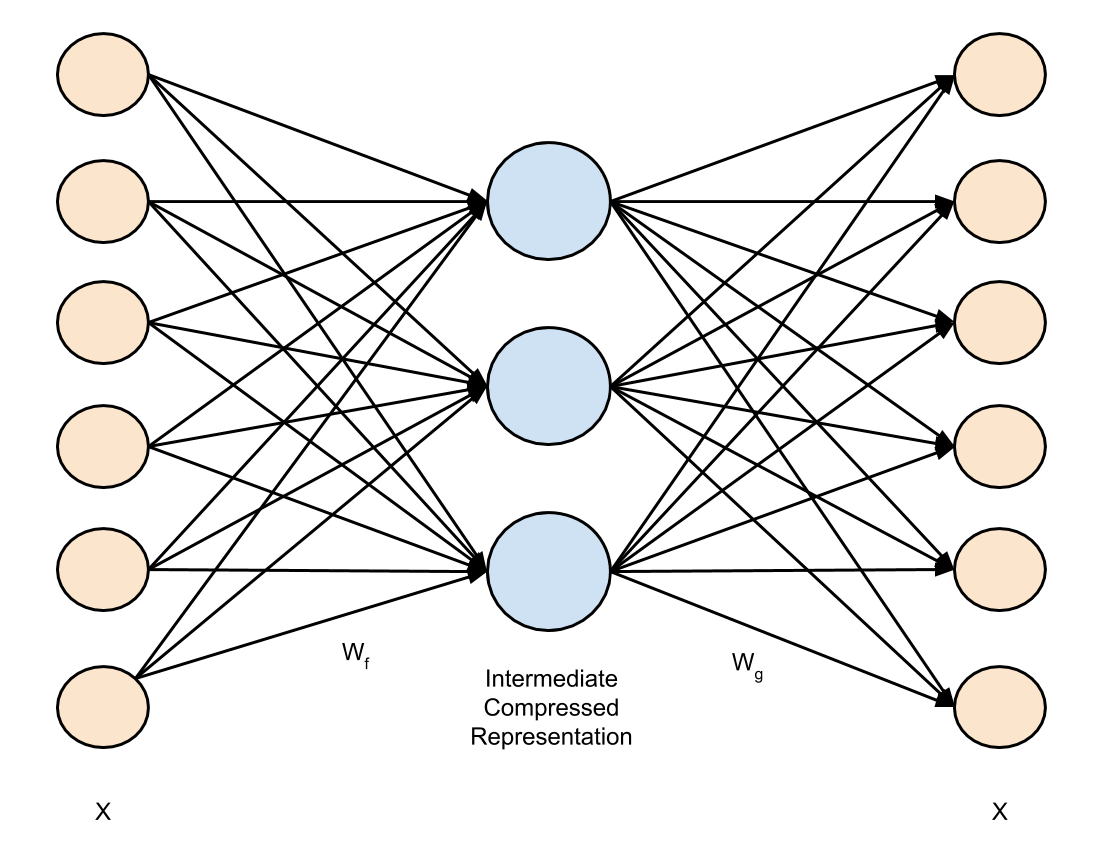
\includegraphics[width=0.7\textwidth]{autoencoders}
            \caption{Autoencoders}
            \label{fig:autoencoders}
        \end{figure}
    \end{itemize}

    \textbf{Linear Autoencoder}
    \begin{itemize}
        \item 
        No activation function involved. The hidden layer is infered from the weights.
        \item 
        $W_g W_f x = x$
        \item 
        $W_g W_f$ would need to be an identity matrix. This derivation is not trivial due to the reduced dimensionality. $W_g$ and $W_f$ are pseudo-inverses of each other.
        \item 
        Deriving the weights using the Euclidean norm objective is equivalent to PCA.
    \end{itemize}

    \textbf{Non-linear Autoencoder}
    \begin{itemize}
        \item 
        Non-linear manifold 
        \item 
        $f$ is a non-linear function that can map data into a lower-dimensional representation. $g$ is another non-linear function that does the exact opposite.
    \end{itemize}

    \textbf{Deep Autoencoder:}
    $f$ and $g$ both consist of multiple layers

    \textbf{Sparse Representation:}
    The hidden layer can be just as large as the input layer, but the loss function penalizes non-zero entries, and tries to create the intermediate representation of the data which is sparse.

    \textbf{Denoising Data:}
    Loss function would use the noisy version as input and the clean version as output.

    \textbf{Probabilistic Autoencoder:}
    Illustration: Figure \ref{fig:autoencoders}.
    \begin{figure}[ht]
        \centering
        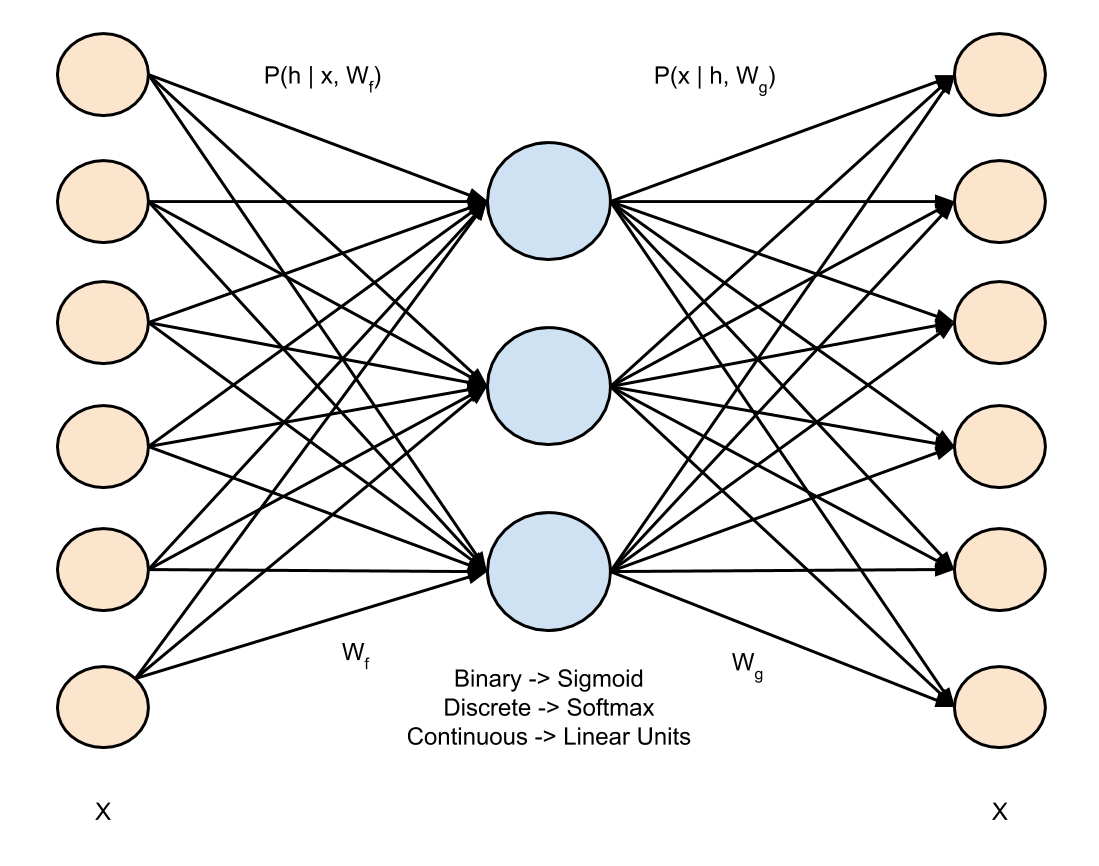
\includegraphics[width=0.7\textwidth]{probabilistic-autoencoder}
        \caption{Probabilistic Autoencoder}
        \label{fig:probabilistic-autoencoder}
    \end{figure}

    \textbf{Generative Model:}
    Sample the hidden `h' and use it as a generative base by which to generate values of `x'.


% section autoencoders (end)


\section{Generative Adversarial Networks} % (fold)
\label{sec:generative_adversarial_networks}

    \begin{itemize}
        \item 
        Similar to Probabilistic Autoencoders, we can use the distribution $P(h)$ to sample new values for $x$.
        \item 
        Problem: how to come up with a $P(h)$?
    \end{itemize}

    \textbf{Variational Autoencoder:}
    \begin{itemize}
        \item 
        The encoded representation $h$ should be a Gaussian distribution with mean 0 and variance 1.
        \item 
        Encoder part of network should approximate the mean and the variance.
        \item 
        Illustration: Figure \ref{fig:variation-autoencoder}.
        \begin{figure}[ht]
            \centering
            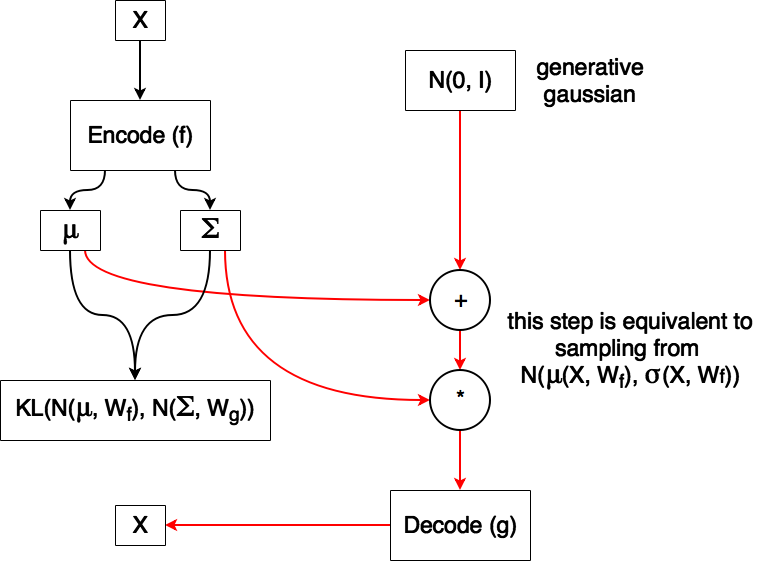
\includegraphics[width=0.7\textwidth]{variation-autoencoder}
            \caption{Variational autoencoder}
            \label{fig:variation-autoencoder}
        \end{figure}
        \item 
        Sampling hinders backpropagation.
    \end{itemize}

    \textbf{Generative Adversarial Network:}
    \begin{itemize}
        \item 
        Game theoretic basis
        \item 
        Generator vs Discriminator (compete; trained simultaneously)
        \item 
        $W_d$ is minimized by a gradient descent algorithm during which $W_g$ remains static.
        Conversely, $W_g$ is maximized by a gradient ascent algorithm during which $W_d$ remains static.
        \item 
        Illustration: Figure \ref{fig:gan-architecture}.
        \begin{figure}[ht]
            \centering
            \includegraphics[width=0.5\textwidth]{gan-architecture}
            \caption{GAN Architecture}
            \label{fig:gan-architecture}
        \end{figure}
    \end{itemize}

% section generative_adversarial_networks (end)


\newpage


\section{Ensemble Learning} % (fold)
\label{sec:ensemble_learning}

    \begin{itemize}
        \item 
        Method to combine several hypotheses into a single stronger hypotheses.
        \item 
        Bagging: Majority voting for a hypothesis, in classification problems
        \item 
        Boosting: Computes a weighted majority
    \end{itemize}

    \textbf{Bagging vs. Boosting}
    \begin{itemize}
        \item 
        Bagging
        \begin{itemize}
            \item 
            Majority vote of a set of hypotheses
            \item
            Assumptions: Hypotheses are independent (error probability independent and roughly the same)
        \end{itemize}
        \item 
        Boosting
        \begin{itemize}
            \item 
            Weighted majority vote
            \item 
            Weighted based on respective error rates
            \item 
            Different hypotheses can be obtained by varying the weight of each datapoint in the training set.
        \end{itemize}
    \end{itemize}

    \begin{figure}[ht]
        \centering
        \includegraphics[width=.4\textwidth]{bagging_independent_classifiers}
        \caption{Bagging - Independent Classifiers}
        \label{fig:bagging_independent_classifiers}
    \end{figure}

    \textbf{Random forests:} Bagging, with decision trees (only classification)

    \textbf{Combining classifier parameters: } Might not always provide the benefits of ensemble learning. Combining the predictions usually proves to be more useful. Refer to Figure \ref{fig:parameter_averaging}. The 2 neural networks are independently accurate at computing the XOR, but averaging the weights yields an incorrect computation.
    \begin{figure}[ht]
        \centering
        \includegraphics[width=.4\textwidth]{parameter_averaging}
        \caption{Parameter Averaging}
        \label{fig:parameter_averaging}
    \end{figure}

% section ensemble_learning (end)


\newpage


\section{Stream Learning} % (fold)
\label{sec:stream_learning}

    \begin{itemize}
        \item 
        Model continuously refreshed as new training data arrives.
        \item 
        Bayesian learning being inherently suited to stream/online learning.
        \item 
        Posterior hypothesis at each point is used as the prior belief for the next point.
        \item 
        To avoid iterating multiple times over the training data, stochastic gradient descent is used.
    \end{itemize}

    \textbf{Robbins-Monro sufficient conditions}
    \begin{itemize}
        \item 
        Choose learning rate $a_n$ such that $\sum_{n=1}^{\infty} a_n = \infty$, but $\sum_{n=1}^{\infty} (a_n)^2 < \infty$
        \item 
        Example of $a_n$ is $\frac{1}{n} $
    \end{itemize}

% section stream_learning (end)


\newpage


\section{Formulae} % (fold)
\label{sec:formulae}

    \begin{itemize}

        \item 
        KNN: 
        $$y_x = mode({y_{x'}| x' \in knn(x)})$$

        \item 
        Weighted KNN (used for regression): 
        $$y_x = \sum_{x' \in knn(x)} w(x, x') y_{x'}$$

        \item 
        Euclidean Loss: 
        $$L(w) = \frac{1}{2} \sum_{n=1}^{N} (y(x_n, w) - t_n)^2 $$

        \item 
        Linear regression Convex Optimization Objective:
        $$w = A^{-1}b$$
        where
        $$A = \sum_{n=1}^{N} \bar{x_n} \bar{x_n}^T$$ and $$b = \sum_{n=1}^{N} t_n \bar{x_n}$$

        \item 
        Regularized Ridge Regression: 
        $$w = argmin_w \frac{1}{2} \sum_{n=1}^{N} (y(x_n, w) - t_n)^2 + \lambda \lVert w \rVert $$
        equivalent to 
        $$w = (\lambda I + A)^{-1}b$$

        \item 
        Joint distribution marginalization
        $$Pr(A = a) = \sum_b Pr(A = a \wedge B = b) $$

        \item 
        Conditional Probability
        $$Pr(A|B) = \frac{Pr(A \wedge B)}{Pr(B)} $$
        implying the chain rule,
        $$Pr(A \wedge B) = Pr(A|B) Pr(B)$$

        \item 
        Bayes Rule:
        $$Pr(B|A) = \frac{Pr(A|B) Pr(B))}{Pr(A)} $$

        \item 
        Bayesian Learning: \\
        Prior: $Pr(H)$ \\
        Likelihood: $Pr(e|H)$ \\
        Evidence: $e = <e_1, e_2, ... e_n>$
        $$Pr(H|e) = k Pr(e|H) Pr(H)$$
        where $k$ is a normalizing constant equivalent to $Pr(e)$ in Bayes Rule

        For a given hypothesis,
        $$Pr(e|h) = \prod_n P(e_n|h)$$

        \item 
        Maximum a posteriori (MAP):
        $$h_{map} = argmax_{h_i} P(h_i|e)$$
        $$h_{map} = argmax_{h_i} P(h) P(e|h_i)$$

        \item 
        Maximum likelihood estimation:
        Same as MAP, except that all the hypotheses have an equal prior probability.
        $$h_{mle} = argmax_{h_i} P(e|h_i)$$
        $$h_{mle} = argmax_{h_i} \sum_n \log P(e_n|h)$$

        \item 
        Gaussian PDF:
        $$\frac{1}{\sqrt{2\pi\sigma}} e^{- \frac{(x - \mu)^2}{2 \sigma^2}}$$

        \item 
        Bias - Variance tradeoff
        $$E[loss] = bias^2 + variance + noise$$

        \item 
        Bayesian Linear Regression:
        $$\bar{w} = \sigma^{-2} A^{-1} \bar{X}^T y $$
        where
        $$A = \sigma^{-2} \bar{X}^T \bar{X} + \Sigma^{-1}$$

        \item 
        Mixture of Gaussians Posterior Distribution:
        $$Pr(C_k|x) = \frac{1}{1 + e^{-(w^Tx + w_0)}}$$
        where
        $$w = \Sigma^{-1} (\mu_k - \mu_j)$$
        $$w_0 = -\frac{1}{2} \mu_k^T \Sigma^{-1} \mu_k + \frac{1}{2} \mu_j^T \Sigma^{-1} \mu_j + \ln\frac{\pi_k}{\pi_j}$$

        \item 
        Mixture of Gaussians MLE Solution:
        $$\pi = \frac{\sum_{n \in c_1} 1}{N}$$
        $$\mu_1 = \frac{\sum_{n \in c_1} x_n}{N}; \mu_2 = \frac{\sum_{n \in c_2} x_n}{N}$$
        $$\Sigma = \frac{S_1 + S_2}{N}$$
        where 
        $$S_1 = \sum_{n \in c_1} (x_n - \mu_1) (x_n - \mu_1)^T; S_2 = \sum_{n \in c_2} (x_n - \mu_2) (x_n - \mu_2)^T$$

        \item 
        Logistic Regression Loss function:
        $$L(w) = - \sum_n y_n \ln \sigma(w^T \bar{x}) + (1 - y_n) \ln (1 - \sigma(w^T \bar{x})) $$

        \item 
        Logistic Regression Gradient descent:
        $$w = w - H^{-1} \nabla L(w)$$
        where H is the Hessian matrix
        $$H = \bar{X} R \bar{X}^T$$
        R is a diagonal matrix with $R_{ii} = \sigma_i(1 - \sigma_i)$ and $\sigma_i = \sigma(w^T \bar{x}_n)$

        \item 
        Perceptron Learning Gradient Descent:
        $$w = w - \eta \nabla E$$
        where $$E = - \sum_{(x_n, y_n) \in M} y_n w^T x_n$$
        and M is a set of misclassified examples and $y \in (1, -1) \forall y$

        \item
        Sigmoid perceptron learning min squared error:
        $$E(w) = \frac{1}{2} \sum_n (y_n - \sigma(w^T x_n))^2 $$
        $Also, \nabla(\sigma) = \sigma(1 - \sigma)$

        \item 
        Multi-layer neural network error function:
        $$E(w) = \frac{1}{2} \lVert f(x_n, W) - y_n \rVert_2^2 $$

        \item 
        Multi-layer neural network Gradient descent
        $$w_{ji} = w_{ji} - \eta \frac{\partial E_n}{\partial w_{ji}} $$

        \item 
        Backpropagation algorithm
        \begin{equation*}
        \delta_j = \left\{
        \begin{array}{@{}ll@{}}
        h'(a_j) (z_j - y_j), & \text{base case, if j is an output unit} \\
        h'(a_j) \sum_k w_{kj}\delta_k, & \text{recursion, if j is a hidden unit}
        \end{array}\right.
        \end{equation*} 

        \item 
        Kernel function:
        $$k(x, x') = \phi(x)^T \phi(x') $$

        \item 
        Weights:
        $$w = - \frac{1}{\lambda} \sum_n (w^T \phi(x_n) - y_n) \phi(x_n) $$
        $$\Phi = [\phi(x_1), \phi(x_2) ... \phi(x_N)] $$
        $$w = \Phi a $$
        $$a_n = - \frac{1}{\lambda} (w^T \phi(x_n) - y_n) $$

        \item 
        Gram matrix
        $$K = \Phi^T \Phi$$
        Optimal $a$
        $$a = (K + \lambda I)^{-1} y $$

        \item 
        Kernel prediction:
        $$y_* = \phi(x_*)^T w $$
        $$y_* = \phi(x_*)^T \Phi a $$
        $$y_* = k(x_*, X) (K + \lambda I)^{-1} y $$
        where $(X, y)$ is the training set and $(x_*, y_*)$ is the test instance

        \item
        Given that $k_1(x, x')$ and $k_2(x, x')$ are valid kernels, the below kernels are valid too
        \begin{itemize}
            \item 
            $ck_1(x, x') \forall c>0 $
            \item 
            $f(x)k_1(x, x')f(x') $
            \item 
            $q(k_1(x, x')) $ where q is a polnomial with co-efficients $\geq 0$
            \item 
            $exp(k_1(x, x')) $
            \item 
            $k_1(x, x') + k_2(x, x')$
            \item 
            $k_1(x, x')k_2(x, x')$
            \item 
            $k_3(\phi(x), \phi(x'))$
            \item 
            $x^T A x'$ where A is symmetric positive semi-definite
            \item 
            $k_a(x_a, x'_a) + k_b(x_b, x'_b)$
            \item 
            $k_a(x_a, x'_a)k_b(x_b, x'_b)$ where $x = \left(\begin{array}{c} x_a\\ x_b\\ \end{array} \right)$
        \end{itemize}

    \end{itemize}

    % section formulae (end)

\end{document}

